\graphicspath{{Chapitre_3/Images/}}
\chapter{Principles of thermodynamics}\label{C3}
%%%%%%%%%%%%%%%%%%%%%%%%%%%%%%%%%%%
%%%%%                         %%%%%
%%%%%Introduction chapitre 2_5%%%%%
%%%%%                         %%%%%
%%%%%%%%%%%%%%%%%%%%%%%%%%%%%%%%%%%
\quad\ The previous chapter covered many concepts to start analyzing a thermodynamic system submitted to various transformations. Among those, the notion of state variables defining the equilibrium state of such system has been defined. 

This chapter will use the first and second principles of the thermodynamic to introduce some state variables that will be used when studying a thermodynamic cycle. Also, a classification of the different transformations will be established.
\section{First principle}
\quad\ The first principle of thermodynamics state that the energy cannot be created or destroyed, but is rather converted from one form to another.
The chapter \ref{C2} shows that for the general case, (\ref{eq:C3_EB}) gives a generic formulation for the energy balance of a system. 

\begin{equation}
  \setstretch{1}
  E_{in} - E_{out} = (Q_{in} - Q_{out}) + (W_{in} - W_{out}) + (E_{mass,in} - E_{mass,out}) = \Delta E_{system} \label{eq:C3_EB}
\end{equation}
\subsection{Enthalpy}
\quad\ Considering a closed system, the third term of the energy balance given in the relation(\ref{eq:C3_EB}) is nullified. Thus, the variation of the total energy from a state \textbf{1} to a state \textbf{2} is given in the relation \ref{eq:C3_EBC}.

\begin{equation}
\setstretch{1}
E_{2} - E_{1} = Q_{1-2} - W_{1-2} = m\cdot\left(u_2 - u_1\right) + \frac{1}{2}m\cdot\left(v^2_2 - v^2_1\right) + m\cdot g\cdot\left(z_2 - z1\right)\citep{Dewallef2019} \label{eq:C3_EBC}
\end{equation}
Let’s note that the terms of kinetic and potential energy are often negligible compared to the internal energy.  

The relation \ref{eq:C3_EBC} can be adapted to be applied for the open system by introducing an accumulation term $\Delta E_{cv}$. This correction allows the following reformulation (\ref{eq:C3_EBO}) of the energy balance.

\begin{equation}
\setstretch{1}
Q_{1-2} - W_{1-2} - E_{2} - E_{1} = \Delta E_{cv}\label{eq:C3_EBO}
\end{equation}
\begin{figure}[h]
\centering
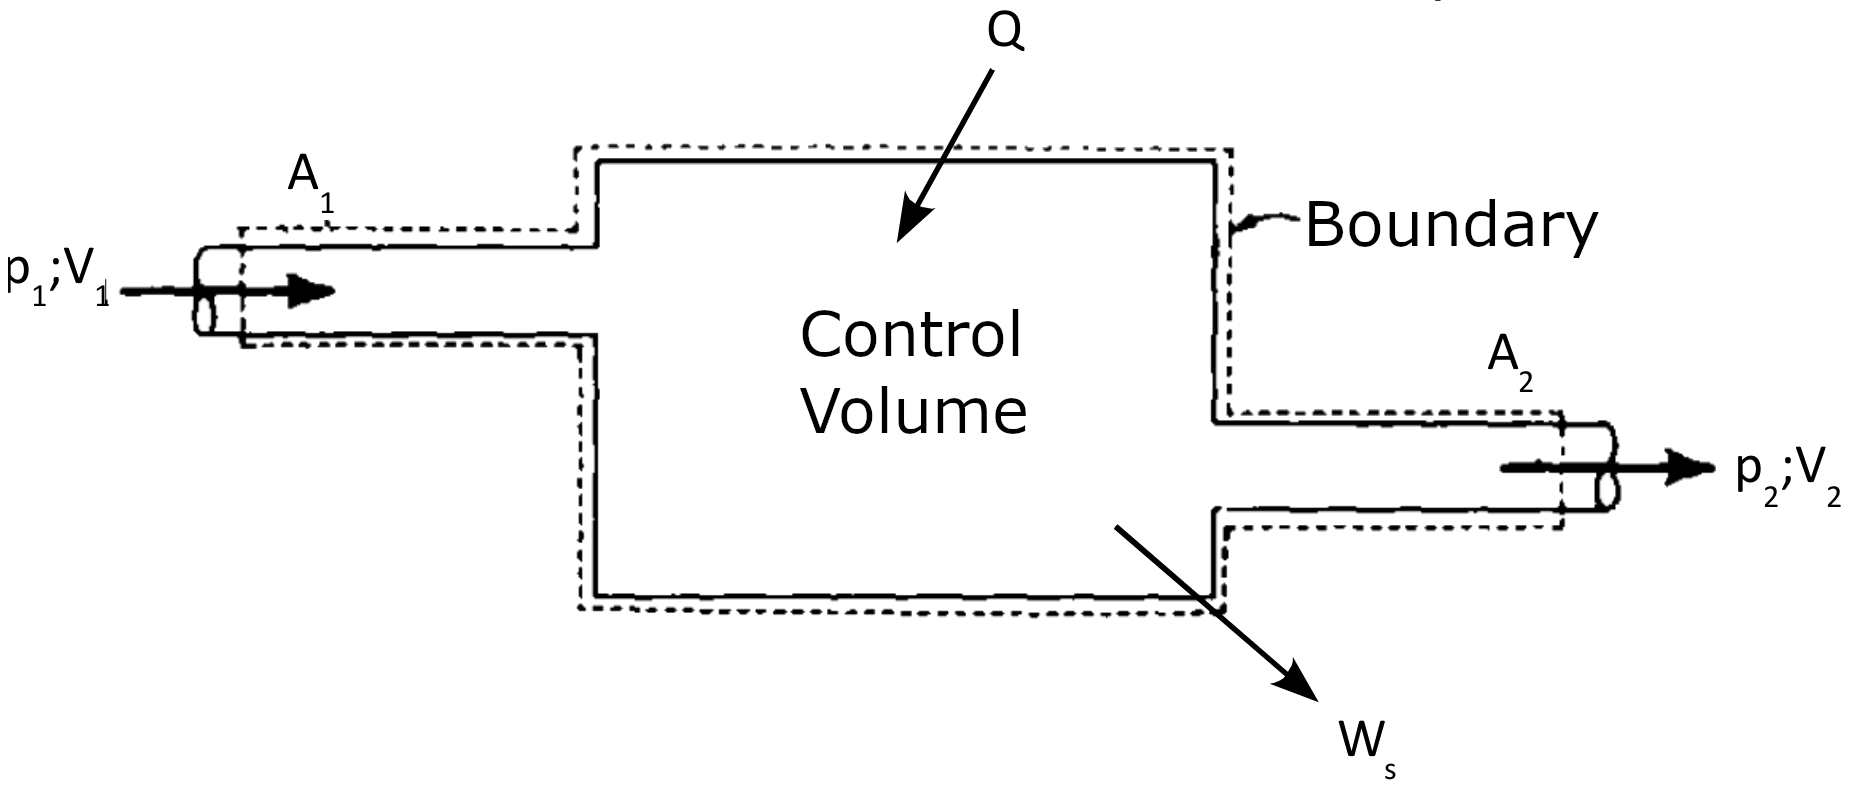
\includegraphics[width=0.7\textwidth]{control_volume.png}
\caption{System control volume \cite{Dewallef2019}.}
\label{fig:C3_VC}
\end{figure}
The Figure \ref{fig:C3_VC} depicts an open system with an inlet and outlet area $A_1$ and $A_2$ respectively. The work $W$ for this system is defined by (\ref{eq:C3_work}).

\begin{equation}
\setstretch{1}
W = p_2\cdot A_2\cdot v_2\cdot \Delta t - p_1\cdot A_1\cdot v_1\cdot \Delta t + W_s \label{eq:C3_work}
\end{equation}      
Where $P$ and $v$ are the pressure and the velocity.

By neglecting the variation of the kinetic and potential energy, the energy balance is after some mathematical operations as given in the relation \ref{eq:C3_EBH}
\begin{equation}
\setstretch{1}
q - w_s = u_2 +p_2\cdot \mathrm{v}_2 - u_1 - p_1\cdot \mathrm{v}_1 = h_2 - h_1\label{eq:C3_EBH}
\end{equation}
Where $q$, $w_s$, and $h$ are respectively the specific work, heat and \textbf{enthalpy} (in J/kg).  

For the case of an ideal gas, the enthalpy and the internal energy only depend on the temperature $T$. Indeed, taking the relation (\ref{eq:C2_GP}) from the previous chapter, the relation (\ref{eq:C3_h}) can easily be deduced.
\begin{equation}
\setstretch{1}
h = u(T) + p\cdot \mathrm{v} = u(T) + r\cdot T \label{eq:C3_h}
\end{equation}
\subsection{Specific heat}
\quad\ The previous subsection was meant to define the enthalpy. This state variable is used in place of the internal energy when dealing with an open system.

Another quantity that is useful for system study is the \textbf{specific heat}. This state variable is defined as the required energy to increase of 1\degree C the temperature of 1 kg of a substance. 
 
The required heat to produce this effect depends on the ways the transformation takes place. For a transformation under constant volume constraints, it is called specific heat at constant volume and denoted $c_v$. If the transformation is performed at constant pressure, the symbol associated with the specific heat is $c_p$.

It is worth noting that the specific heat at constant pressure is always higher than the $c_v$. When performing the transformation at constant pressure, the gas expands against the external pressure. This means that the gas does work and, this is the reason behind the greater value of the supplied heat when dealing with a transformation at constant pressure. 

For an ideal gas, the variation of the internal energy can be linked to the specific heat at constant volume as written in the relation (\ref{eq:C3_UC}).

\begin{equation}
\setstretch{1}
du = c_vdT \rightarrow u_2 - u_1 = \int_{T_1}^{T_2} c_vdT\label{eq:C3_UC}
\end{equation} 
Similarly, the variation of the enthalpy can be expressed using the specific heat at constant pressure.

\begin{equation}
\setstretch{1}
dh = c_pdT \rightarrow h_2 - h_1 = \int_{T_1}^{T_2} c_pdT\label{eq:C3_UP}
\end{equation} 
These two relations, with the equality (\ref{eq:C3_h}), provide the required tools to express the gas constant $r$ as a function of the temperature only. 

\begin{equation}
\setstretch{1}
r = c_p - c_v \label{eq:C3_r}
\end{equation}

Aside the gas constant, the specific heat ratio $k$ (\ref{eq:C3_k}) is also a useful variable to be computed.
\begin{equation}
\setstretch{1}
k = \frac{c_p}{c_v} \label{eq:C3_k}
\end{equation}
\subsection{Carnot cycle}
\quad\, The previous subsections used the first principle of the thermodynamic to deduce two useful state variables, namely the enthalpy and the specific heat.

Now, let’s move aside those notions and let consider the case where the transformation applied to a system is reversible. A necessary condition for the reversibility is that the transformation has to be done in quasi-equilibrium. This implies that if the transformation is reversed, the system goes back to its initial state.

\begin{figure}[h]
\centering
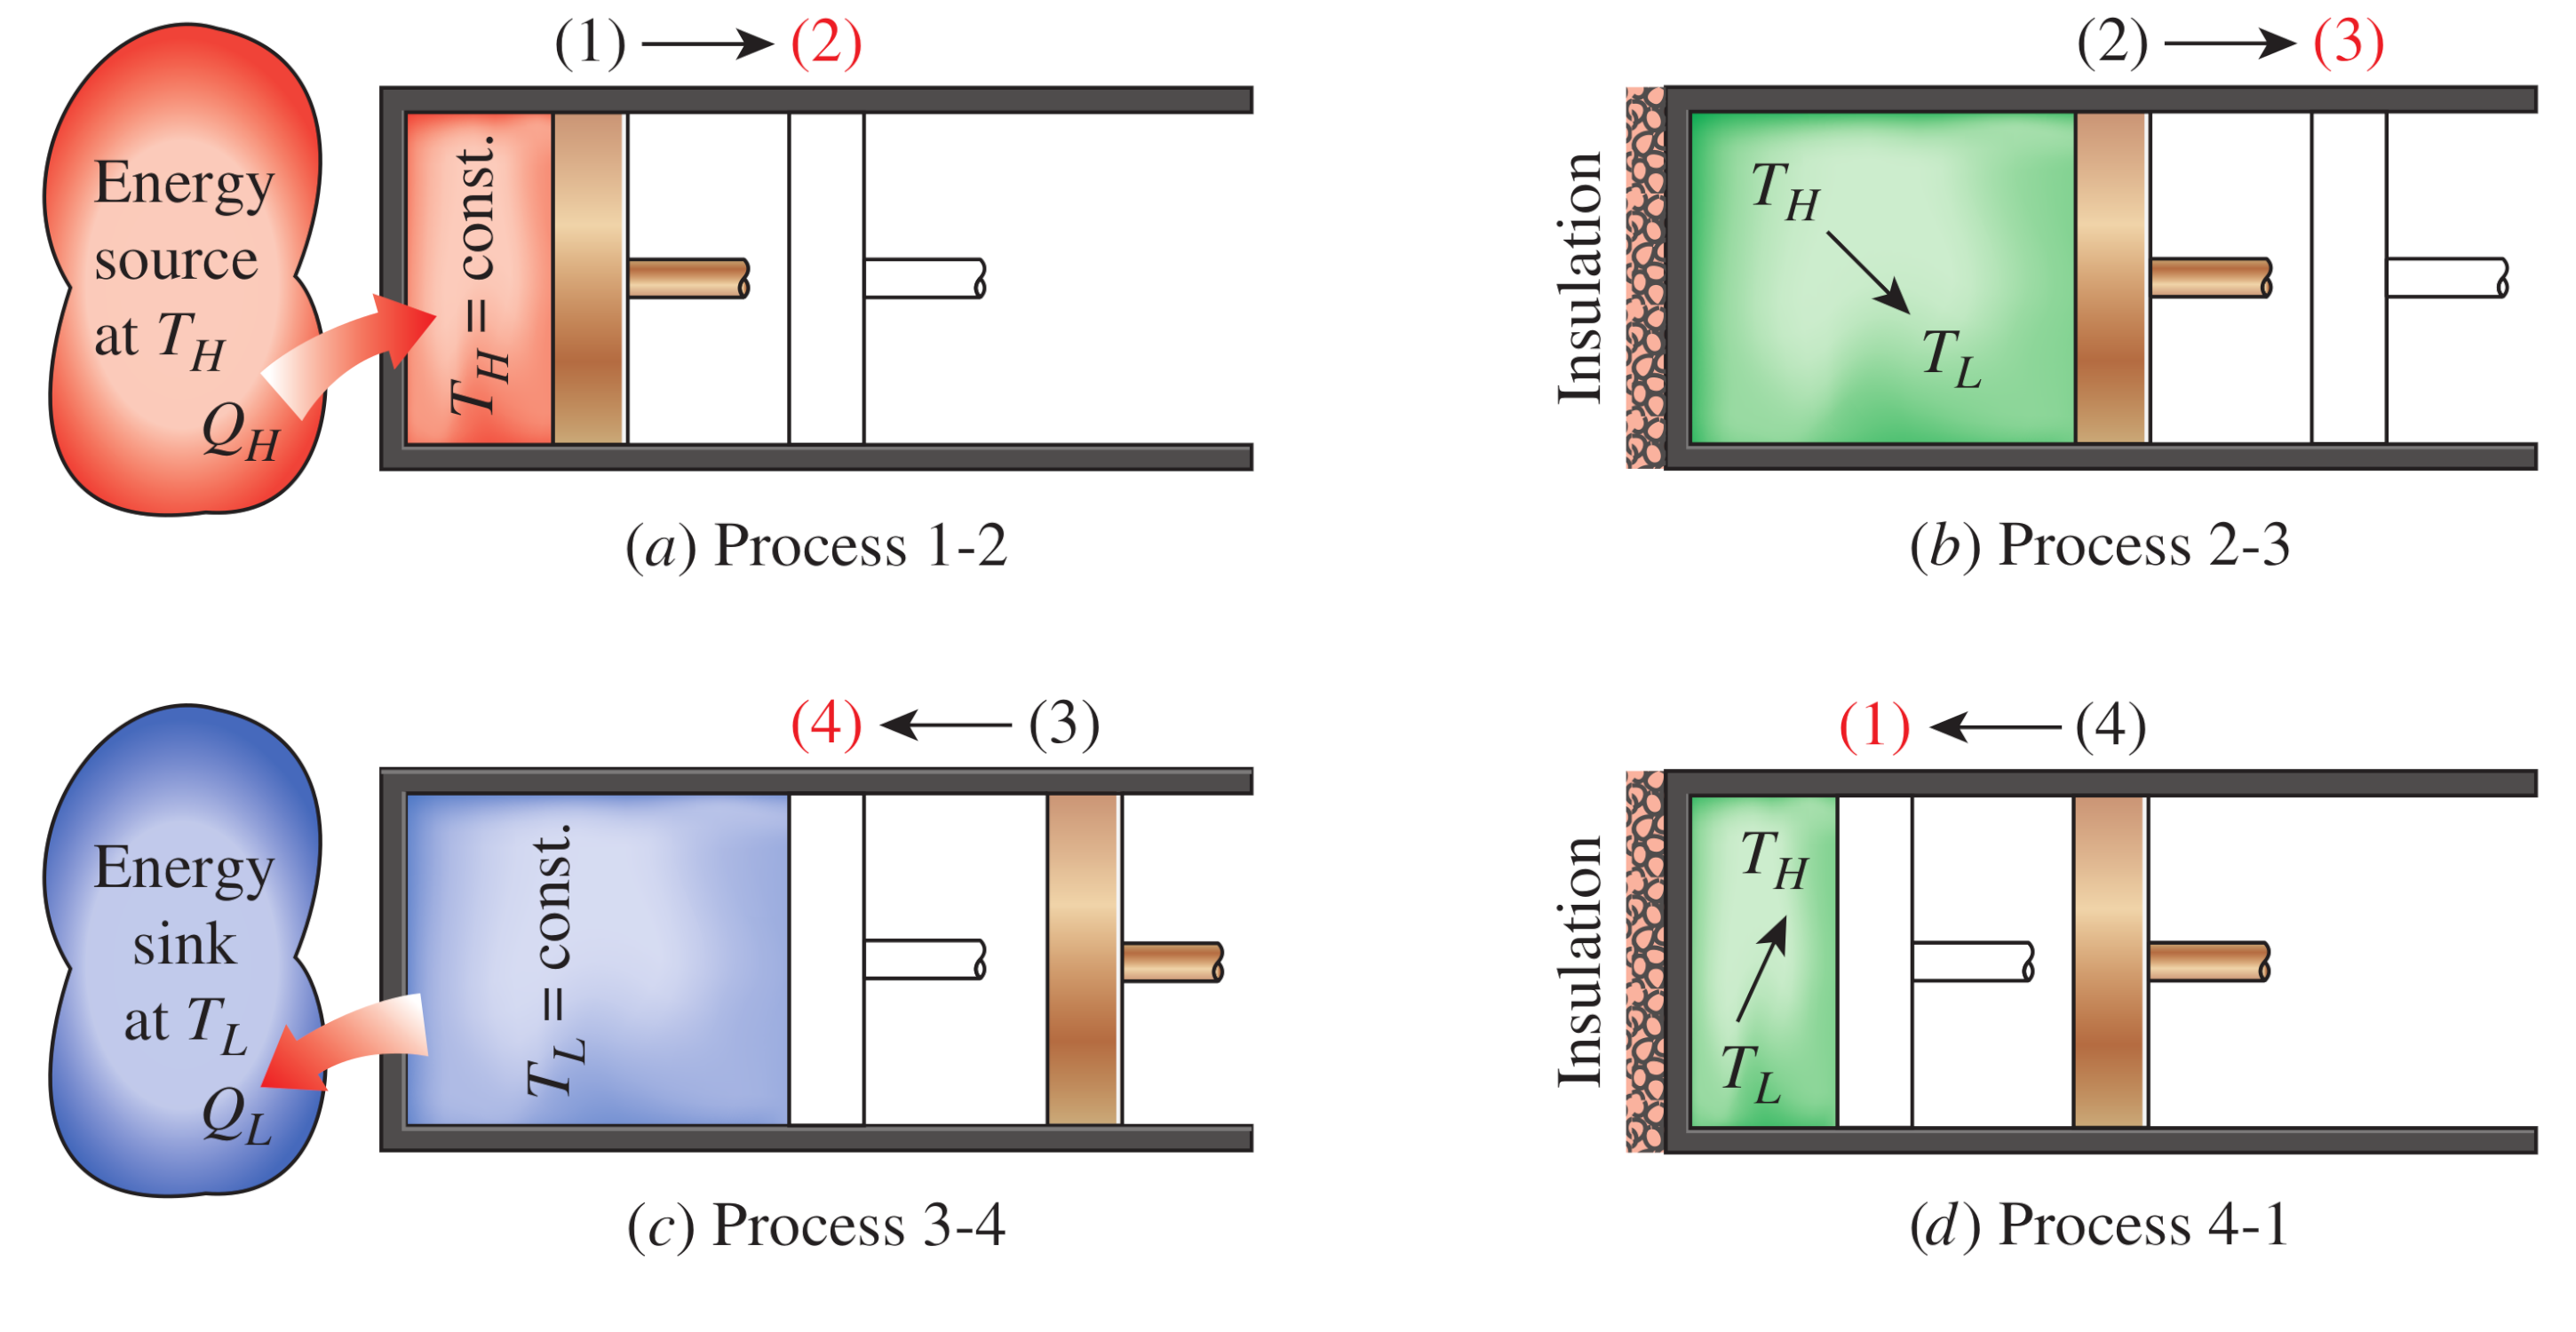
\includegraphics[width=0.7\textwidth]{Carnot_schema.png}
\caption{Carnot cycle - Schematic \cite{2015}.}
\label{fig:C3_Carnot}
\end{figure}

The Carnot cycle is a thermodynamic cycle composed of 4 reversible transformations illustrated in Figure \ref{fig:C3_Carnot}. The transformations are defined as follows.

\begin{itemize}
\setstretch{1}
\item \textbf{1} to \textbf{2} (Figure \ref{fig:C3_Carnot}a): Reversible isothermal expansion with a heat transfer $Q_H$ from the environment to the system
\item \textbf{2} to \textbf{3} (Figure \ref{fig:C3_Carnot}b): Reversible  adiabatic expansion
\item \textbf{3} to \textbf{4} (Figure \ref{fig:C3_Carnot}c): Reversible isothermal compression with a heat transfer $Q_L$ from the system to the environment
\item \textbf{4} to \textbf{1} (Figure \ref{fig:C3_Carnot}d): Reversible adiabatic compression
\end{itemize}
For visual representation, this cycle has been represented in the PV diagram \ref{fig:C3_CarnotPV} where the different transformations are illustrated.
\begin{figure}[h]
\centering
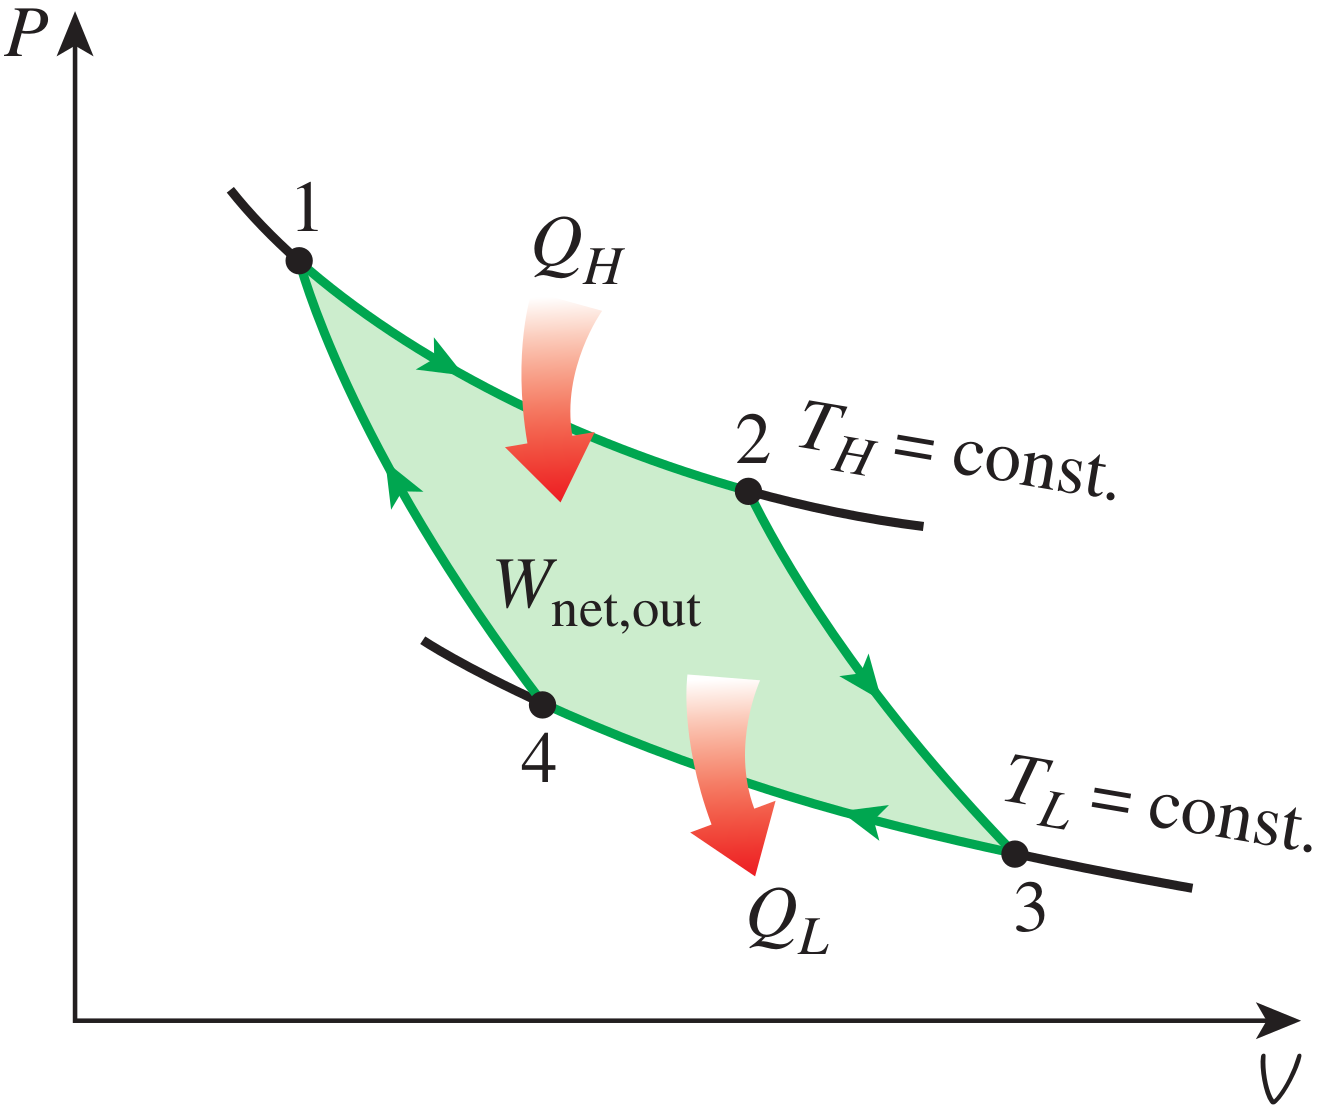
\includegraphics[width=0.5\textwidth]{Carnot_PV.png}
\caption{Carnot cycle - PV diagram \cite{2015}.}
\label{fig:C3_CarnotPV}
\end{figure}
Using the first principle, the net work provided by the cycle is equal to $W_{net,out}=Q_H-Q_L$. From this result and the definition of the efficiency in chapter \ref{C2}, the efficiency of the Carnot cycle is given in (\ref{eq:C3_Carnoteff}).

\begin{equation}
\setstretch{1}
\eta_{carnot} = \frac{W_{net,out}}{Q_H} = 1 - \frac{Q_H}{Q_L}\label{eq:C3_Carnoteff}
\end{equation} 
Considering that the working fluid is an ideal gas, it can be demonstrated that the heats $Q_H$ and $Q_L$ can be replaced by the corresponding temperature $T_H$ of the hot source and $T_C$ of the cold sink.

\begin{equation}
\setstretch{1}
\eta_{carnot}=1-\frac{T_H}{T_L}\label{eq:C3_eff_carnot}
\end{equation} 
The efficiency of the Carnot cycle is optimal. This implies that for any system playing with a hot source $T_H$ and a cold sink $T_C$, its efficiency cannot be greater than the Carnot efficiency with the \textbf{same} hot source and cold sink temperatures.
\subsection{Entropy}
\quad\ The last lines explained that a system with a hot source $T_H$ and a cold sink $T_C$ will never have a efficiency greater than the Carnot efficiency (for the same source and sink).

It has been demonstrated in 1865 by the German physicist R. J. E. Clausius that "the cyclic integral $\oint\frac{\delta Q}{T}$ is always less than or equal to zero."\cite{2015}

\begin{equation}
\setstretch{1}
\oint\frac{\delta Q}{T} = \frac{Q_H}{T_H} - \frac{Q_L}{T_L}\leq 0\label{eq:C3_cyc}
\end{equation}
For the Carnot cycle, the integral is equal to zeros because the two ratios $\frac{Q_H}{Q_L}$ and $\frac{T_H}{T_L}$ are equal.
From the definition \ref{eq:C3_cyc} can be defined a new state variable named \textbf{entropy}. The entropy S is always measured based on a reference point and, its expression is given in the relation (\ref{eq:C3_S}).

\begin{equation}
\setstretch{1}
dS \triangleq \frac{\delta Q_{rev}}{T}\label{eq:C3_S}
\end{equation}
Where $\delta Q_{rev}$ is the "infinitesimal quantity of heat exchanged in a reversible way between the system and the environment at the temperature T."\cite{Dewallef2019} 

For a reversible adiabatic transformation, the $\delta Q_{rev}=0$. This implies that the entropy remains constant. Such transformations are called \textbf{isentropic} transformation.
\begin{figure}[h]
\centering
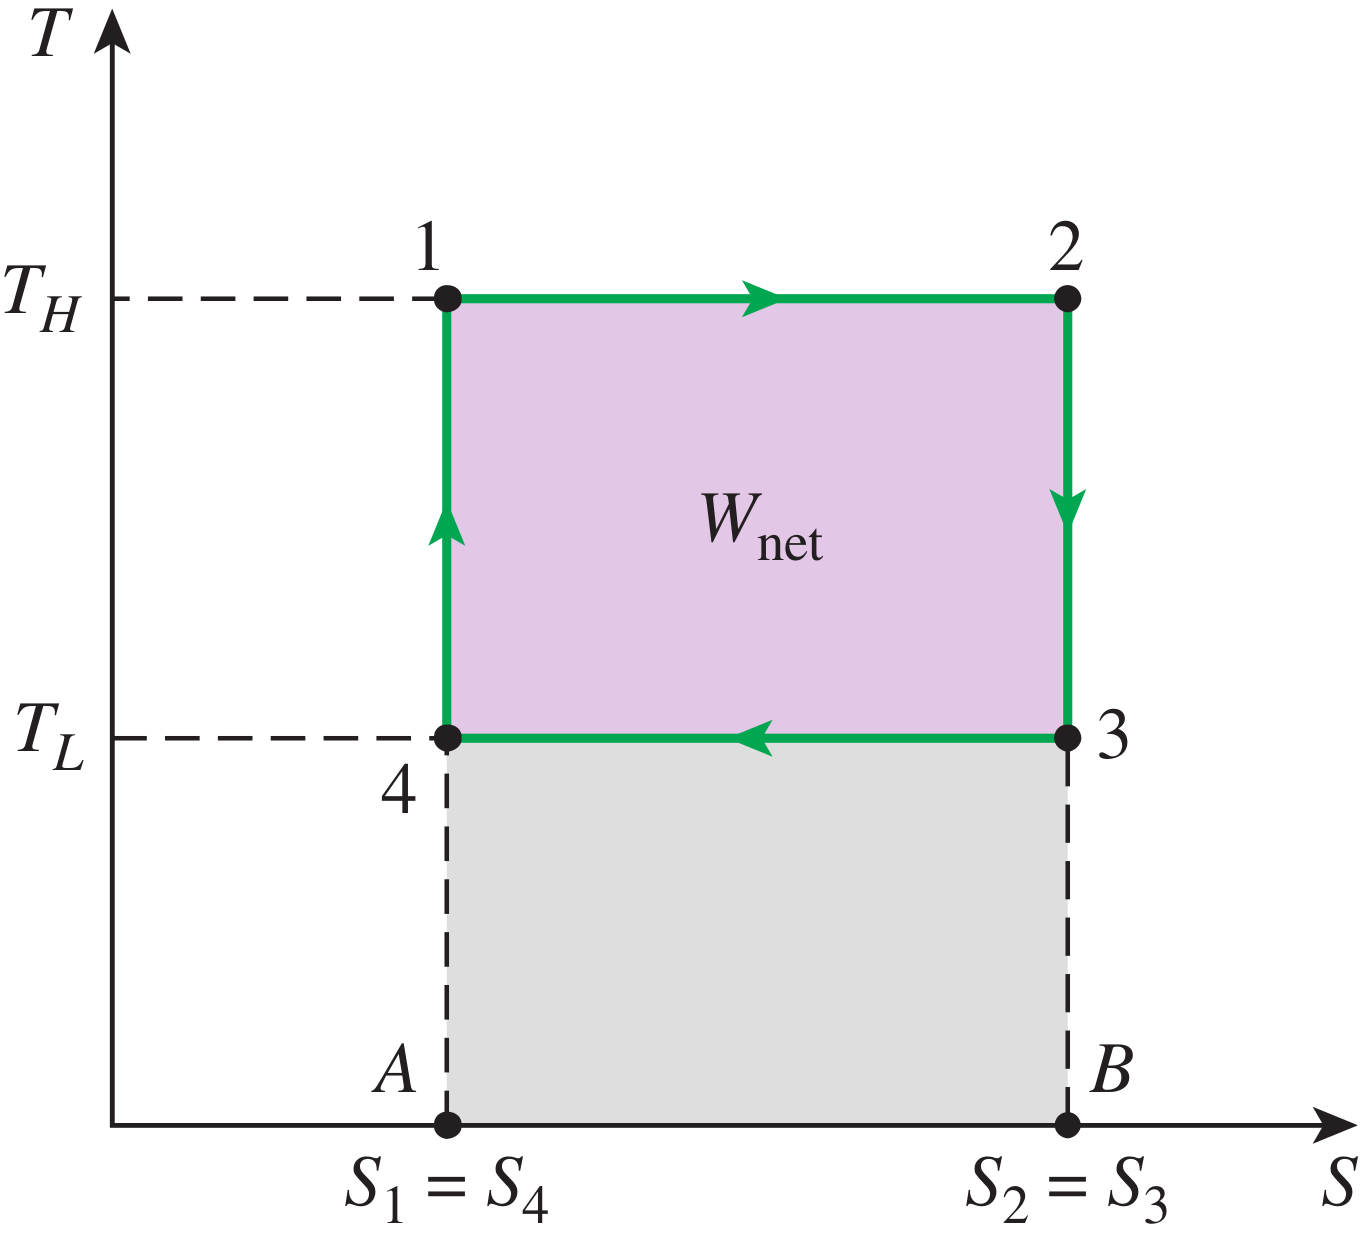
\includegraphics[width=0.5\textwidth]{Carnot_TS.png}
\caption{Carnot cycle - TS diagram \cite{2015}.}
\label{fig:C3_CarnotTS}
\end{figure}
\section{Second principle}
\quad\, Defining the entropy gives a great tool to measure the "quality" of the transformation compared to a similar but reversible transformation.

Based on this definition, one formulation of the second principle of the thermodynamic is that for every transformation, the entropy of the final state of any isolated system is greater or equal to the one of the initial state.

Considering the system defined in the previous lines, it can be said that the increase of entropy $\Delta S_L$ of the cold sink has to be at least greater than the diminution of entropy $\Delta S_H$ of the hot source.

In the case of the Carnot cycle, both variations are equal. This is illustrated on the TS diagram \ref{fig:C3_CarnotTS} where the entropy of states \textbf{1} and \textbf{2} are respectively equal to the entropy of states \textbf{4} and \textbf{3}.
\section{Type of transformations}
\quad\ During this chapter, it has been mentioned several times the notions of reversible processes. 

As it has been explained, a transformation is said reversible if it takes an infinite amount of time to bring the system from its initial state \textbf{1} to its final state \textbf{2}. The different types of transformation are going to be described in the section.\newpage
\subsection{Isothermal transformation}
\begin{wrapfigure}{r}{0.3\linewidth}
  \centering
  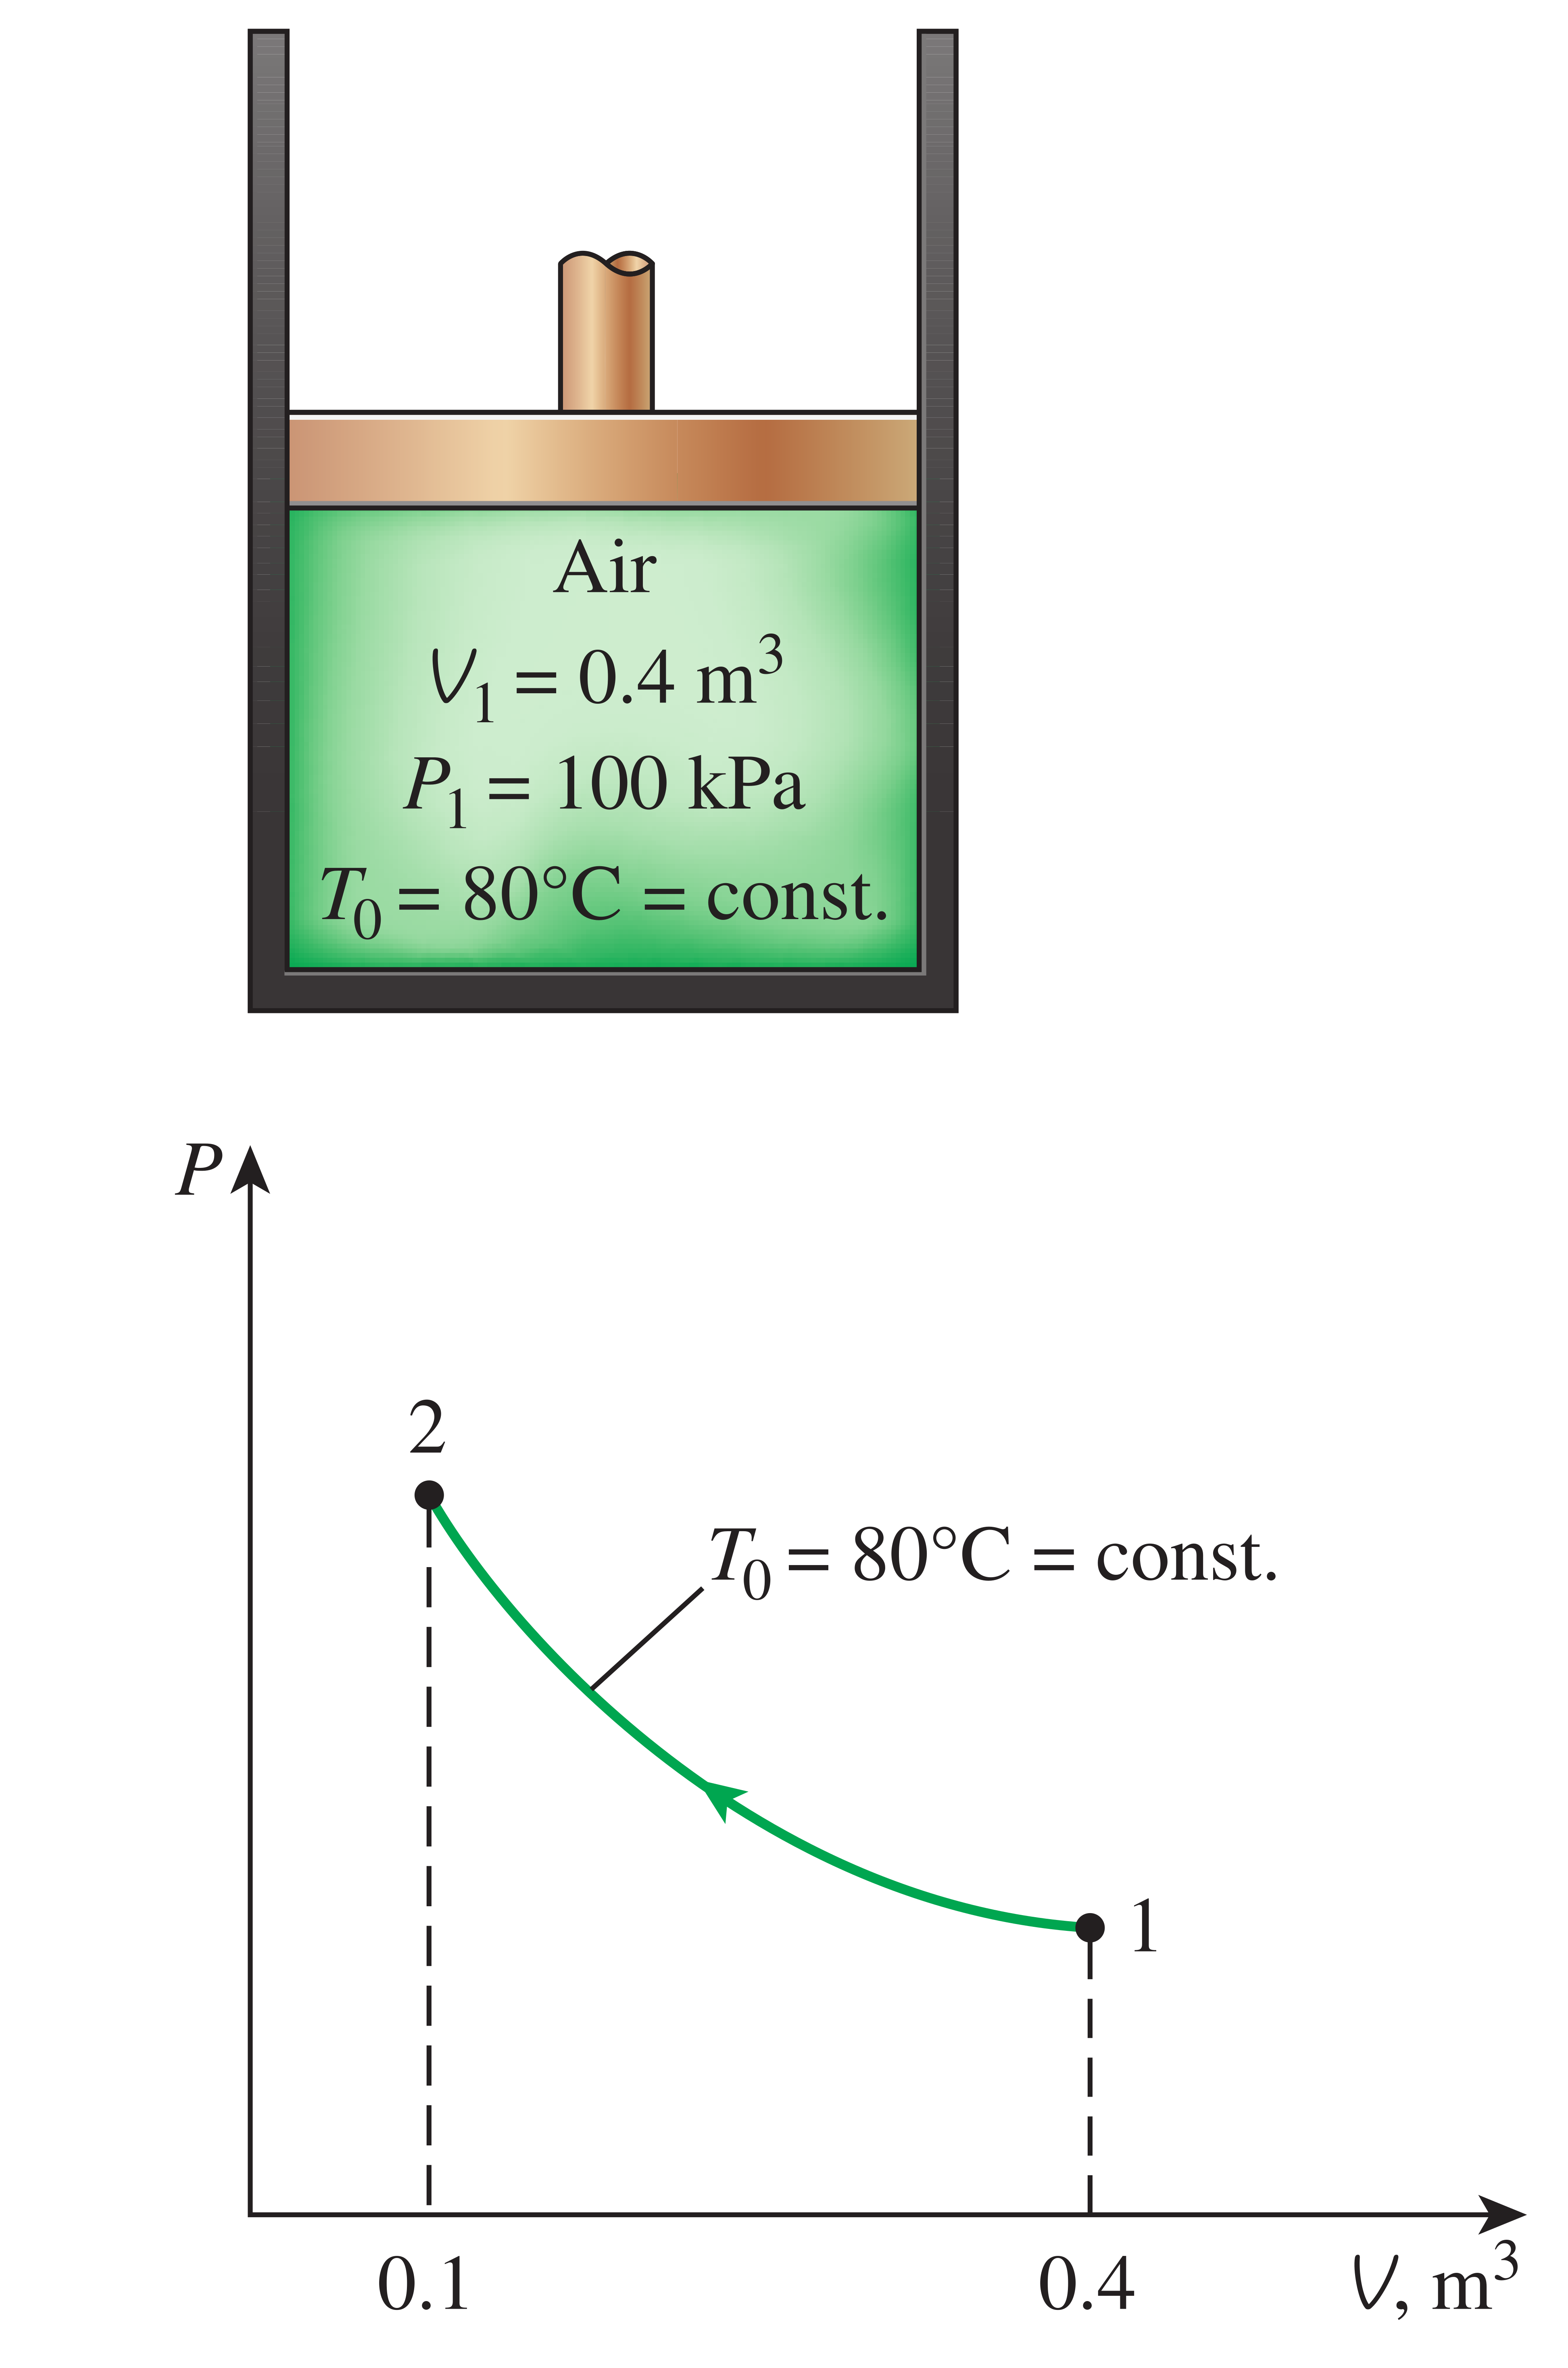
\includegraphics{isoT.png}
  \caption{Isothermal transformation \cite{2015}.}
  \label{fig:C3_isoT}
  \end{wrapfigure}
\quad\ The first type of transformations to be considered are the isothermal processes. Here, since the transformation brings the system from states \textbf{1} to \textbf{2}, the equality \(T_2 = T_1\)  is enforced. 

The transformation is said reversible isothermal if during all the processes the temperature remains constant. Such transformation is depicted in Figure \ref{fig:C3_isoT}. The ideal gas equation (\ref{eq:C2_GP}) allows deriving the relation (\ref{eq:C3_isoT}) if the mass within the system does not vary.

\setstretch{1}
  \begin{align}
    p_1\cdot \mathrm{V}_1 &= p_2\cdot \mathrm{V}_2\nonumber\\
    \rightarrow p\cdot \mathrm{V} &= C \label{eq:C3_isoT}  
  \end{align}
\setstretch{1.5}

 For a compression or expansion, the process is said isothermal if the system is respectively cooled heat up to bring the final state temperature to its initial value.
 
Considering an isothermal compression, the boundary work $W_b$, corresponding to the area below the curve, is given in the development (\ref{eq:C3_WbisoT})

\begin{wrapfigure}{r}{0.3\linewidth}
  \centering
  \includegraphics{poly.png}
  \caption{Polytropic transformation \cite{2015}.}
  \label{fig:C3_poly}
\end{wrapfigure}
 \setstretch{1}
\begin{align}
  W_b &= \int_1^2 pd\mathrm{V} = C\cdot\int_1^2d\mathrm{V}\nonumber\\
  &= C\cdot \ln \frac{V_2}{V_1} = p_1\cdot V_1\cdot \ln \frac{V_2}{V_1} \label{eq:C3_WbisoT}
\end{align}
\subsection{Polytropic transformation}
 \setstretch{1.5}
\quad\ The polytropic transformation, depicted in Figure \ref{fig:C3_poly}, is  a generalization of the isothermal transformation. For an ideal gas, the polytropic transformation is characterized by the relation (\ref{eq:C3_poly}).
  \setstretch{1}
\begin{equation}
  p\cdot \mathrm{V}^n = C \label{eq:C3_poly}
\end{equation}
\setstretch{1.5}
Where $n$ is a constant. 
For $n=1$, the transformation simply corresponds to the isothermal transformation.\clearpage
 
\subsection{Isobaric transformation}
\begin{wrapfigure}{l}{0.3\linewidth}
  \centering
  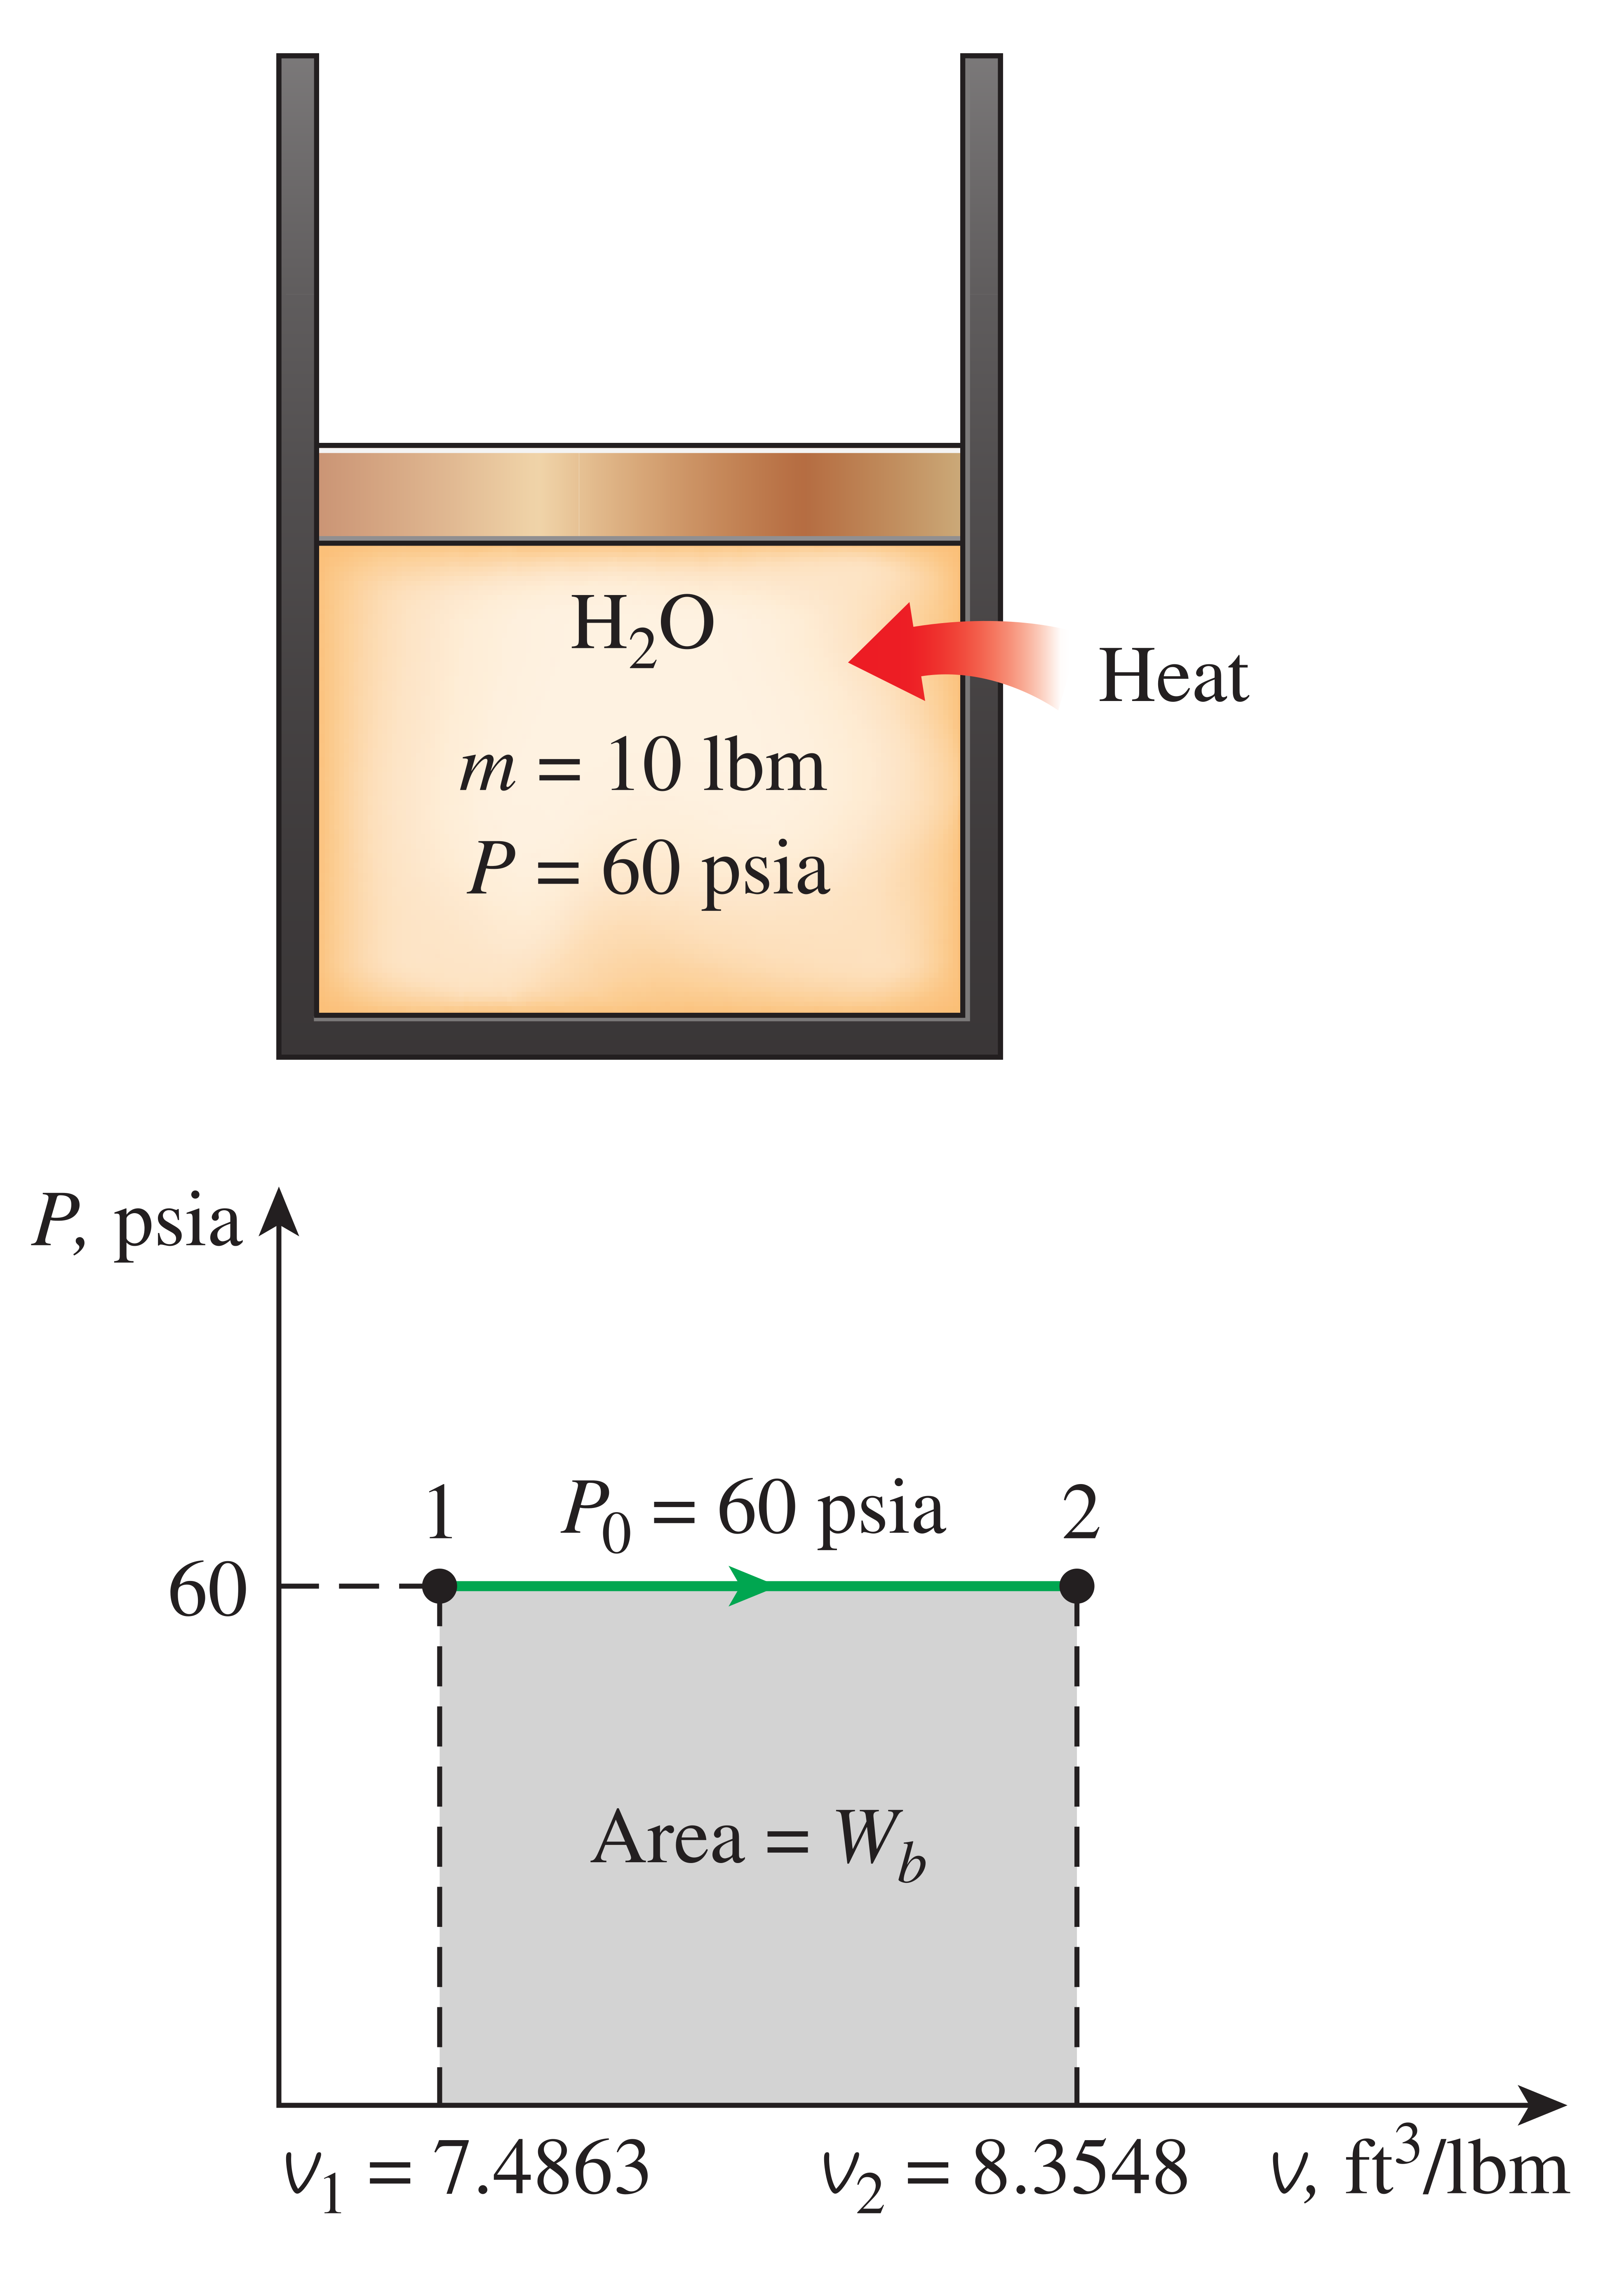
\includegraphics{isoP.png}
  \caption{Isobaric transformation \cite{2015}.}
  \label{fig:C3_isoB}
\end{wrapfigure}
\quad\ The isobaric transformation is one for which the initial and final state are both characterized by the same pressure. Thus, the equality \(p_2 = p_1 = p_0\). 

The figure \ref{fig:C3_isoB} illustrates such transformation.
Typically, the transformation within the combustion chamber, heat exchanger or piping aim to be as close as this transformation. 

Diverging from this ideal transformation implies that the component induces some pressure losses.

As for the isothermal transformation, the boundary work for an isobaric transformation is equal to the area below the curve. Here, the expression is given in the equation (\ref{eq:C3_WbisoP}).

  \setstretch{1}
\begin{align}
  W_b &= p_0\cdot \int_1^2d\mathrm{V}\nonumber\\
   &= p_0\cdot (\mathrm{V_2} - \mathrm{V_1}) = m\cdot p_0\cdot (\mathrm{v_2} - \mathrm{v_1}) \label{eq:C3_WbisoP}
\end{align}

\subsection{Isentropic transformation}
\setstretch{1.5}
\quad\ The last transformation to be considered is the isentropic transformation. This transformation corresponds to a reversible adiabatic transformation. 

Typically, when considering the expansion or the compression of a fluid, the manufacturers aim to build a machine which tends to minimize as much as possible the irreversibilities. 

\begin{figure}[h]
  \centering
  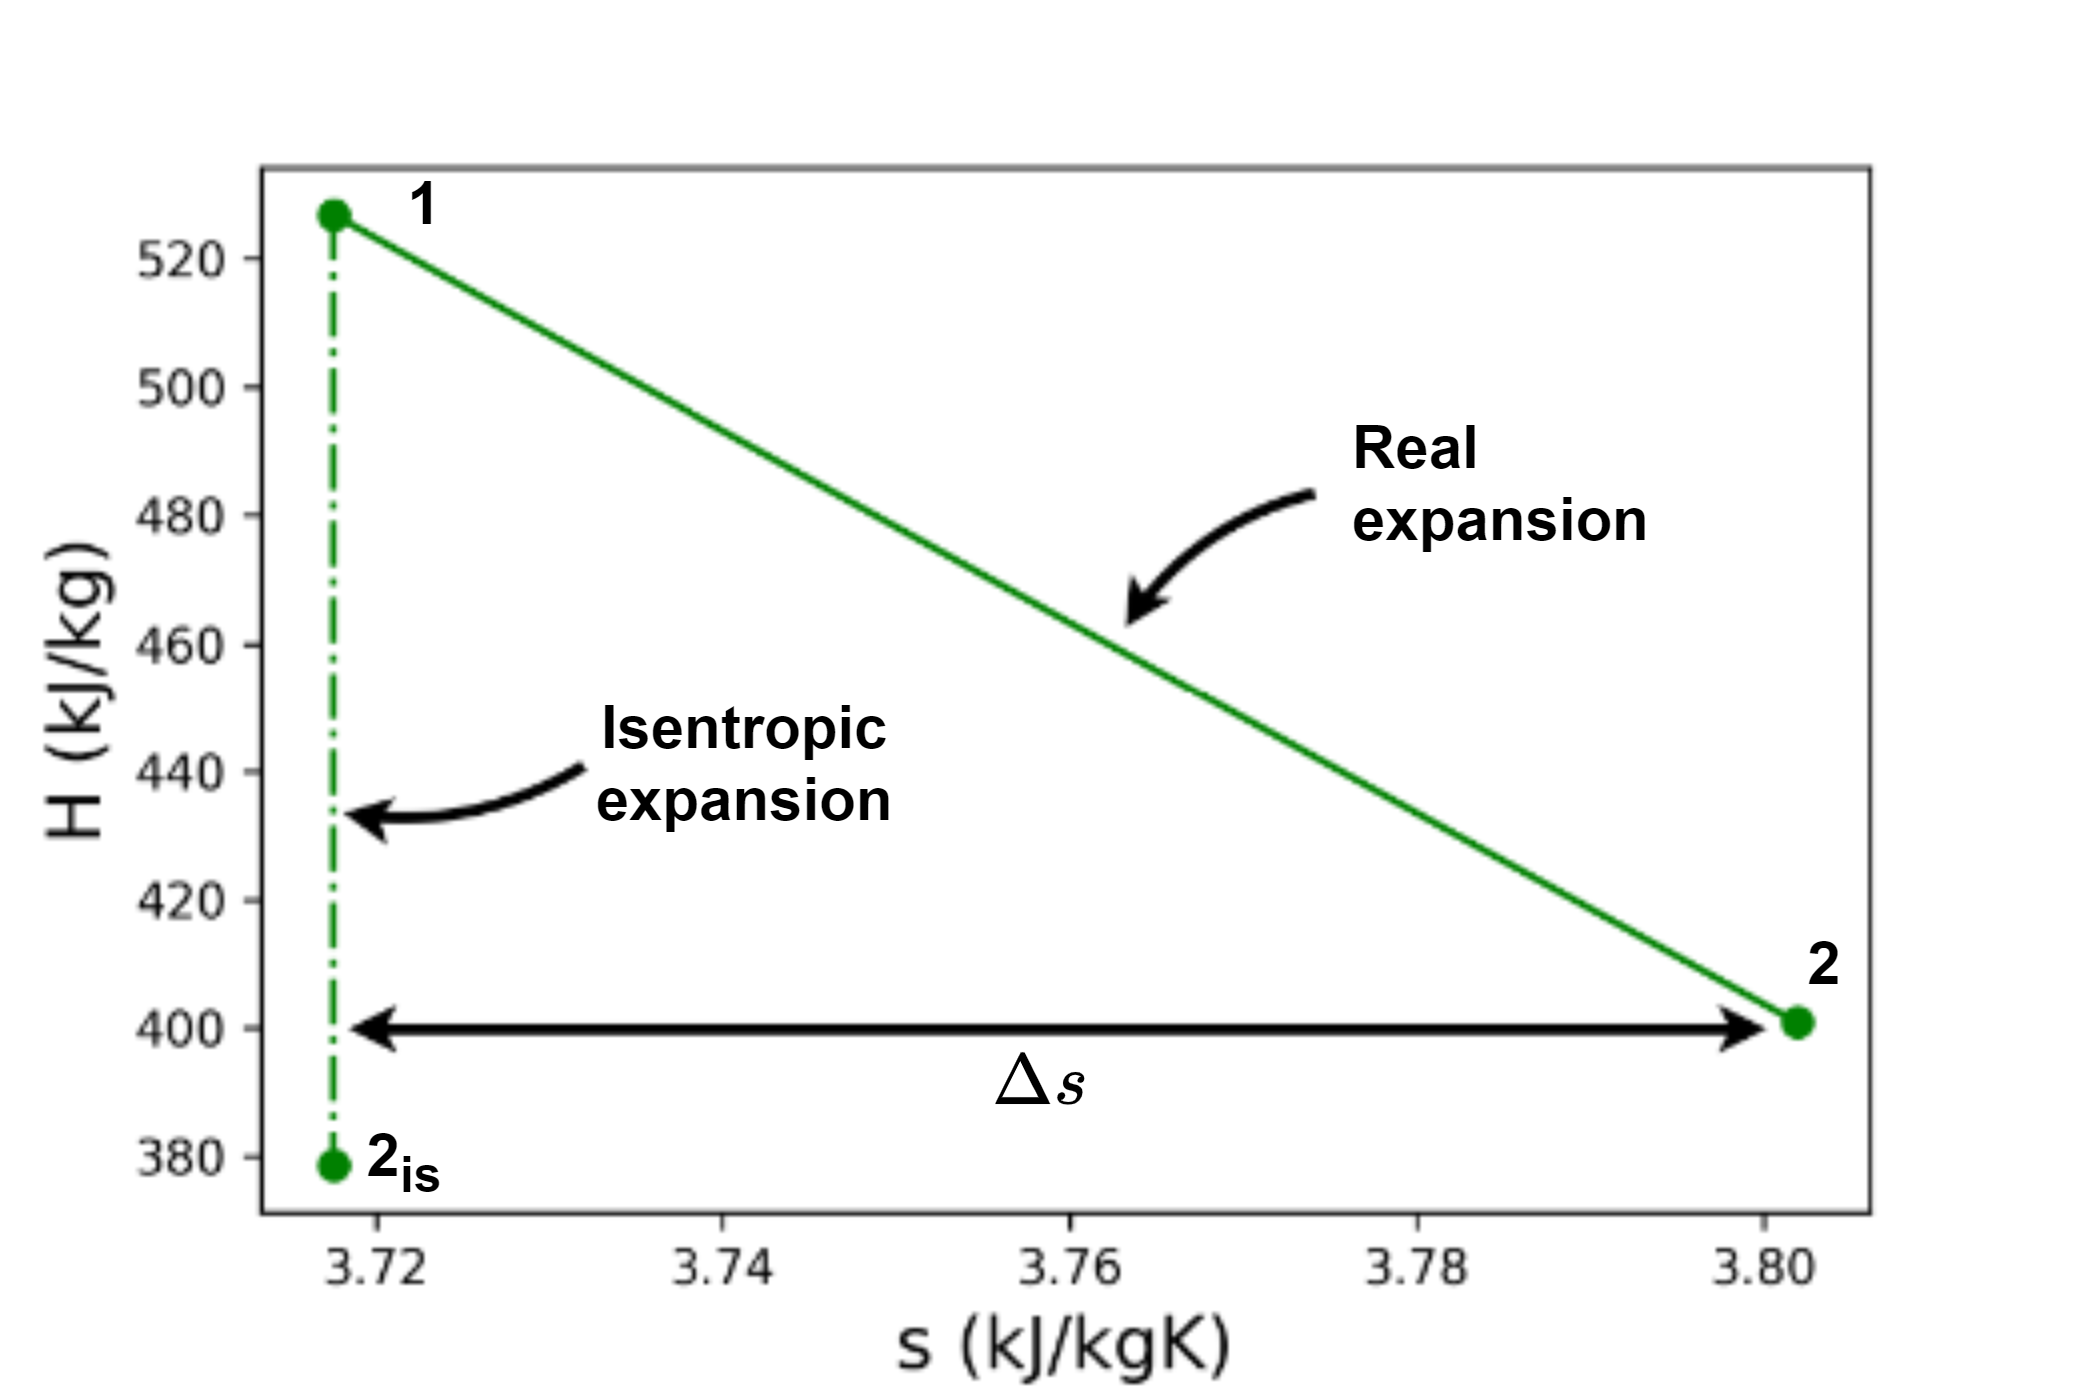
\includegraphics[width=0.6\textwidth]{expansion.png}
  \caption{Isentropic and real expansion.}
  \label{fig:C3_expansion}
\end{figure}
In Figure \ref{fig:C3_expansion} is depicted an isentropic and a real expansion. As it can be noticed, the real expansion produces an augmentation of the entropy of the system. 

Moreover, the isentropic expansion is more efficient since the energy (in term of enthalpy) extracted from the fluid is higher compared to the real expansion. The subscript "is" emphasizes the final state of the isentropic transformation.

It can be demonstrated that the enthalpy at the state \textbf{2$_{is}$} is lower than the enthalpy at the state \textbf{2}. The consequence is that more work have been produced during the transformation. 
\section{Computation of the thermodynamic properties}
\quad\, From now, the hypothesis of an ideal gas has been used for the computation of the previously established state variables. However, while this hypothesis remains quite valid when dealing with gas, it cannot be used for a real fluid (e.g. liquid water).

This problem can be solved using the Maxwell relations which provides a linked between the partial derivatives of the state variables $p$, $v$, $T$ and $s$ for a simple compressible system \cite{2015}. 

Those relations can be derived from the four Gibbs relations expressed in (\ref{eq:C3_Gibbs}).

\begin{subequations}
\setstretch{1}
\begin{equation}
  du = Tds - pdv \label{eq:C3_Gibbs1} 
\end{equation}    
\begin{equation}
  dh = Tds + vdp \label{eq:C3_Gibbs2} 
\end{equation}
\begin{equation}
  da = du - Tds - sdT = - pdv - sdT \label{eq:C3_Gibbs3} 
\end{equation}    
\begin{equation}
  dg = dh - Tds - sdT = vdp - sdT \label{eq:C3_Gibbs4}
\end{equation} \label{eq:C3_Gibbs}
\end{subequations}
where the state variables $a$ and $g$ are the Helmholtz and Gibbs function (respectively).
Analyzing the relations allows to notice that each of them are of the form

\begin{align}
\setstretch{1}
dz &= Mdx + Ndy\label{eq:C3_Maxbase}\\
\text{with } \left.\frac{\partial M}{\partial y}\right|_x &= \left.\frac{\partial N}{\partial x}\right|_y\label{eq:C3_partMax}
\end{align}
Using this property, the links between the different state variables are easily obtained by applying the relation (\ref{eq:C3_partMax}) to the equations (\ref{eq:C3_Gibbs1}) to (\ref{eq:C3_Gibbs4}).

\begin{subequations}
\setstretch{1}
\begin{equation}
  \left.\frac{\partial T}{\partial v}\right|_s =  - \left.\frac{\partial p}{\partial s}\right|_v \label{eq:C3_Max1} 
\end{equation}    
\begin{equation}
  \left.\frac{\partial T}{\partial p}\right|_s = \left.\frac{\partial v}{\partial s}\right|_p \label{eq:C3_Max2}  
\end{equation}
\begin{equation}
  \left.\frac{\partial s}{\partial v}\right|_T = \left.\frac{\partial p}{\partial T}\right|_v \label{eq:C3_Max3} 
\end{equation}    
\begin{equation}
  \left.\frac{\partial s}{\partial p}\right|_T =  - \left.\frac{\partial v}{\partial T}\right|_p \label{eq:C3_Max4} 
\end{equation} \label{eq:C3_Max}
\end{subequations}
The relations (\ref{eq:C3_Max}) are called Maxwell equations are helpful in thermodynamics. They provide a method to calculate the variation of the entropy of a system based on the measurement of the variation of the pressure, volume and temperature.

However, this method for calculating the thermodynamic variables is limited to simple compressible system and cannot be used when the system involves "electrical, magnetic, and other effects"\cite{2015}.

These are the relations used when using a digital library for the thermodynamic assessment of the state of a pure fluid with real properties. The open-source library named \textbf{CoolProp}\cite{Bell2014} is one of the best known and. In this work, the library will be called many time when the ideal gas approximation is not relevant.
\section{Entropy variation}
\quad\, The previous section introduced the four equations of state (\ref{eq:C3_Gibbs1}) to (\ref{eq:C3_Gibbs4}). Among those, the second equation allows to write the relation (\ref{eq:C3_ds}).
\begin{equation}
ds = c_p\frac{dT}{T} - r\frac{dp}{p}\label{eq:C3_ds}
\end{equation}

By performing the integration over the path of a transformation going from state \textbf{1} to state \textbf{2}, the relation (\ref{eq:C3_s}) gives the link between the entropy variation and the temperature and pressure variation between the two states.

\begin{equation}
\setstretch{1}
s_2 - s_1  = \int_1^2\frac{c_p}{T}dT - r\cdot ln\frac{p_2}{p_1}\label{eq:C3_s}
\end{equation}
Supposing that the variation of the specific heat with respect to temperature is negligible, the development (\ref{eq:C3_Deltas}) can be derived. 

\begin{equation}
\setstretch{1}
s_2 - s_1= r\cdot \left(\frac{k}{k-1}\cdot ln\frac{T_2}{p_1} - ln\frac{p_2}{p_1}\right) = r\cdot ln\left[\frac{p_1}{p_2}\cdot\left(\frac{T_2}{T_1}\right)^\frac{k}{k-1}\right] \label{eq:C3_Deltas}
\end{equation}
Where the $c_p=\frac{r\cdot k}{k-1}$ by using the two relations (\ref{eq:C3_r}) and (\ref{eq:C3_k}).

For an isentropic process, the equality $s_2=s_1$ is enforced. Thus, from (\ref{eq:C3_Deltas}) the relations (\ref{eq:C3_isrelPT}) and (\ref{eq:C3_isrelrhoT}) are obtained.

\begin{subequations}
\setstretch{1}
\begin{equation}
\frac{p_2}{p_1} = \left(\frac{T_2}{T_1}\right)^\frac{k}{k-1}\label{eq:C3_isrelPT}
\end{equation}
\begin{equation}
\frac{\rho_2}{\rho_1} = \left(\frac{T_2}{T_1}\right)^\frac{1}{k-1}
\label{eq:C3_isrelrhoT}
\end{equation}
\label{eq:C3_isrel}
\end{subequations}
\section{Isentropic efficiency} \label{C3:Isen_eff}
\quad\, For any real transformations, there is always an augmentation of the entropy when the system goes from its initial state \textbf{1} to its final state \textbf{2}. This implies that the difference $s_2 - s_1$ is greater than zero.

This can be characterized by defining the isentropic efficiency as being the image of the irreversibilities induced by the transformation. this type of efficiency is very frequently used when studying the compression or the expansion of a fluid.

For a compression or an expansion, the isentropic efficiency is defined by stating that the pressure ratio $\frac{p_1}{p_2}$ is the identical for both the isentropic and non isentropic transformation. Let's substituting this ratio by the constant $\Pi$. 

Considering first the ideal case, the equation (\ref{eq:C3_isrelPT}) gives after a reordering of the term the relation (\ref{eq:C3_Tis}).

\begin{equation}
\setstretch{1}
T_{2,is} = T_1\cdot\Pi^\frac{k-1}{k}\label{eq:C3_Tis}
\end{equation}

Then, for the real transformation, the left-hand-side of the relation (\ref{eq:C3_Deltas}) is greater than zero. This implies that the temperature at the end of the real transformation is always greater than the one at the en of the isentropic transformation. Thus, it leads to (\ref{eq:C3_T}).

\begin{equation}
\setstretch{1}
T_{2} > T_{2,is} = T_1\cdot\Pi^\frac{k-1}{k}\label{eq:C3_T}
\end{equation}
As can be noticed, the real transformation leads to a final state temperature bigger than for the isentropic transformation. This difference allows to define the isentropic efficiency $\eta_{is}$. The definition varies based on the desired transformation
\begin{itemize}
\setstretch{1}
\item Compression: $\eta_{is}=\frac{T_{2,is}-T_1}{T_2-T_1}=\frac{h_{2,is}-h_1}{h_2-h_1}$
\item Expansion: $\eta_{is}=\frac{T_1-T_{2}}{T_1-T_{2,is}}=\frac{h_1-h_{2}}{h_1-h_{2,is}}$
\end{itemize}
Where the temperature and the enthalpy variation provide the same output result due to the ideal gas hypothesis. 

For real fluid, the only valid definition of the isentropic efficiency is the one based on the enthalpy variation. 